\section{Model and Training Objective}
\label{sec:method}

\begin{figure*}[t]
  \centering
  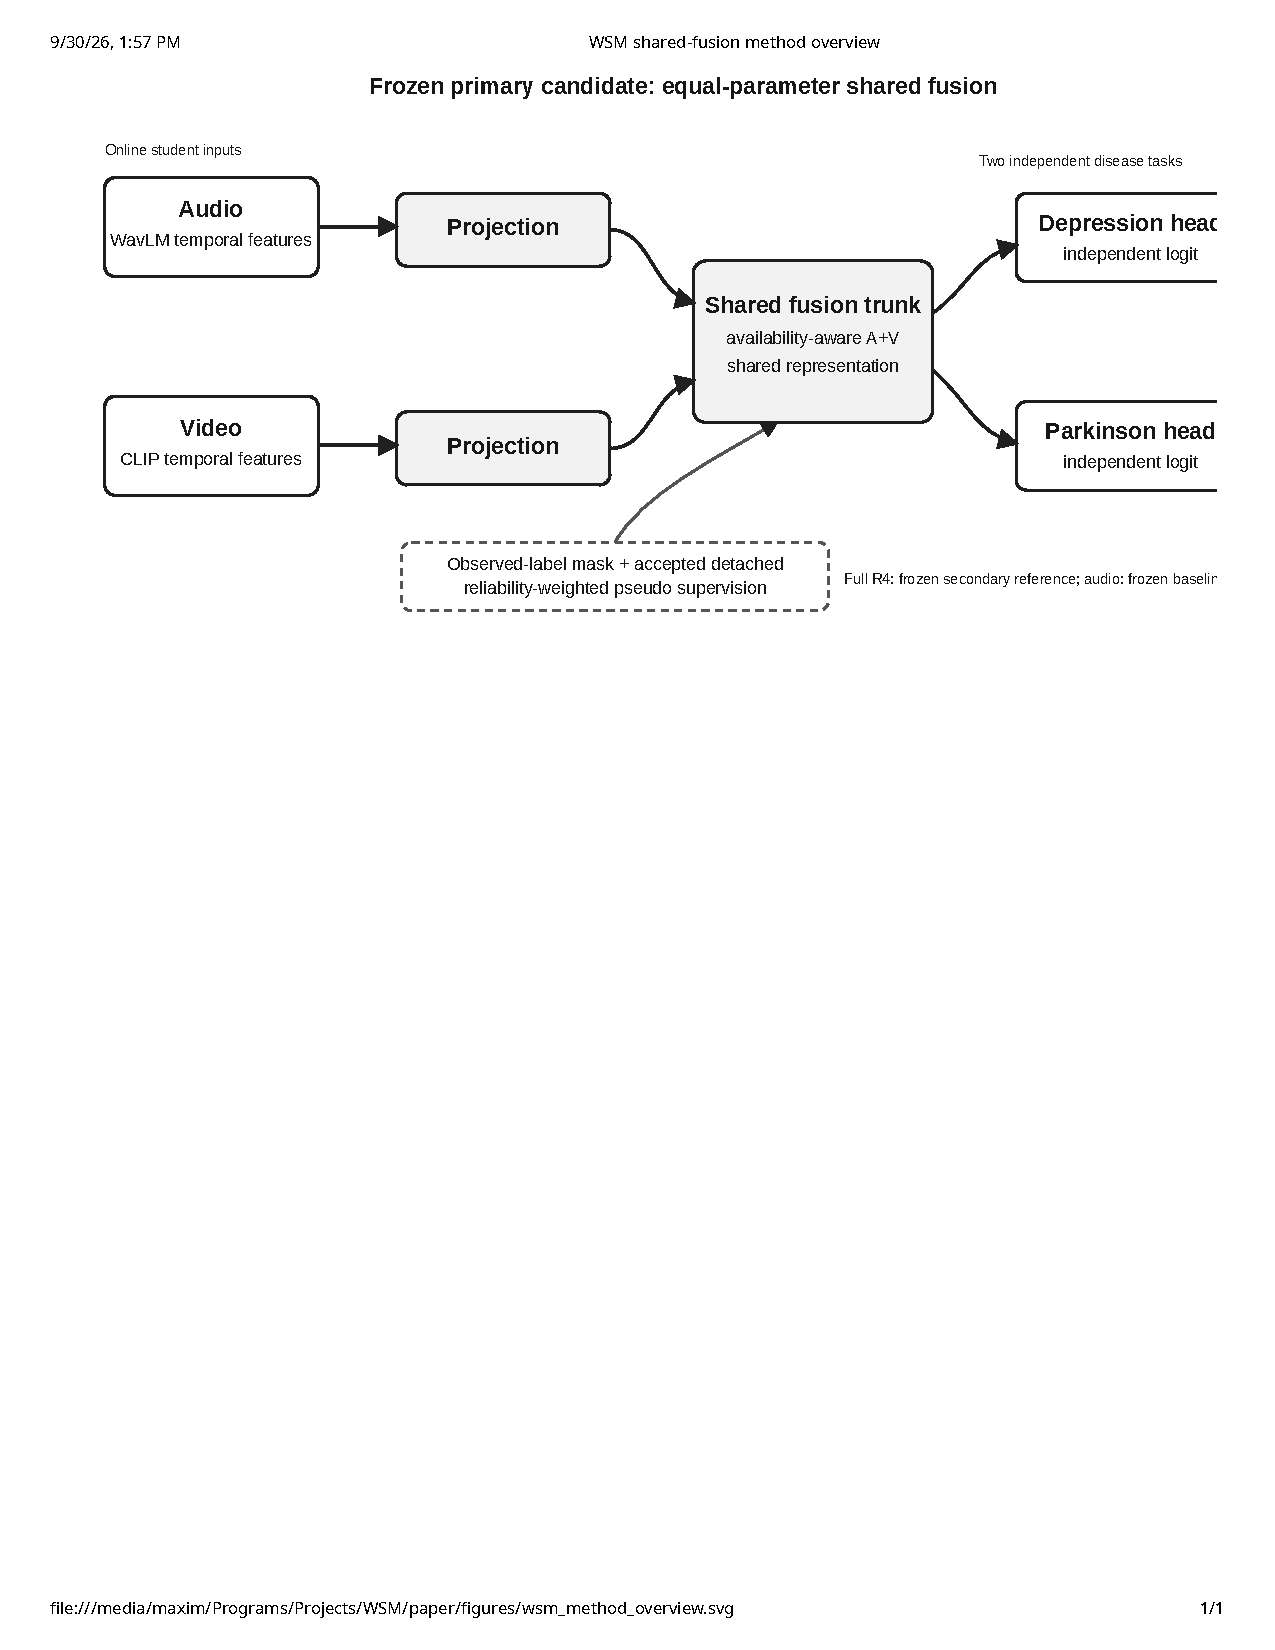
\includegraphics[width=0.88\textwidth]{figures/wsm_method_overview.pdf}
  \caption{Two-panel vector overview of the primary equal-parameter shared-fusion model and its frozen training recipe. Solid arrows denote inference; dashed arrows are training-only supervision paths. Full R4 changes shared query/candidate/gating/fusion to task-specific versions but has the same trainable parameter count (295,239). RA-STCH is retained in the frozen recipe; its contribution is not supported by the Stage-6 ablation.}
  \label{fig:overview}
\end{figure*}

\subsection{Availability-aware shared fusion}

The primary model is the frozen disease-query architecture with \texttt{task\_aware\_fusion=false}. Let $x_a$ be the online audio class representation, and let $X_v$ and $m_v$ be temporal video features and their valid-position mask. With projections $P_a,P_v$ and masked temporal pooling,
\begin{equation}
 h_a=P_a(x_a),\qquad
 h_v=P_v\!\left(\frac{\sum_jm_{vj}X_{vj}}{\max(1,\sum_jm_{vj})}\right).
 \label{eq:project}
\end{equation}
An unavailable modality is zeroed before projection and its projected feature is also masked after projection. Consequently the corresponding gate weight is zero and no unavailable modality feature is introduced as a fabricated signal.

The implementation begins with two learned disease queries $q_D,q_P$, but the primary model uses their mean:
\begin{equation}
 \bar q=\tfrac12(q_D+q_P).
\end{equation}
Let $\mathrm{LN}_t$ be the two candidate normalizations. Its shared modality candidates are
\begin{equation}
\begin{aligned}
 c_a&=\tfrac12\sum_{t\in\{D,P\}}\mathrm{LN}_{t}(h_a+\bar q),\\
 c_v&=\tfrac12\sum_{t\in\{D,P\}}\mathrm{LN}_{t}(h_v+\bar q).
\end{aligned}
 \label{eq:candidates}
\end{equation}
A shared gate $g$ scores the query--candidate concatenations:
\begin{equation}
 s_a=g([\bar q;c_a]),\qquad s_v=g([\bar q;c_v]).
\end{equation}
For availability vector $\mathbf a=(a_a,a_v)$, unavailable scores are set to $-\infty$ before the softmax:
\begin{equation}
 (\alpha_a,\alpha_v)=\operatorname{softmax}_{\mathbf a}(s_a,s_v).
 \label{eq:gate}
\end{equation}
The fused feature first combines candidates and then averages the two fusion normalizations,
\begin{equation}
\begin{aligned}
 u&=\bar q+\alpha_ac_a+\alpha_vc_v,\\
 h&=\tfrac12\sum_{t\in\{D,P\}}\mathrm{LN}^{f}_{t}(u),\qquad z_t=f_t(h).
\end{aligned}
 \label{eq:fuse}
\end{equation}
The two output heads $f_D,f_P$ remain independent sigmoid-logit heads. Full R4 instead retains a separate $q_t$, $c_{a,t}$, $c_{v,t}$, gate, and fused representation for each task. Both models have exactly 295,239 trainable downstream parameters; the shared model is a simplification in conditioning, not a reduction in model size.

\subsection{Masked multi-component objective}

For task $t$, observed mask $m_{it}$, accepted pseudo mask $a_{it}$, logits $z_{it}$, and BCE-with-logits $\ell$, the observed component is
\begin{equation}
 L_{\mathrm{obs},t} =
 \frac{\sum_i m_{it}\ell(z_{it},y_{it})}{\sum_i m_{it}+\epsilon}.
 \label{eq:obs}
\end{equation}
For missing accepted entries, $\tilde y_{it}$ and $r_{it}$ are detached pseudo target and reliability:
\begin{equation}
 L_{\mathrm{pseudo},t} =
 \frac{\sum_i(1-m_{it})a_{it}r_{it}\ell(z_{it},\tilde y_{it})}
 {\sum_i(1-m_{it})a_{it}r_{it}+\epsilon}.
 \label{eq:pseudo}
\end{equation}
This operation does not turn unaccepted entries into negatives. The cache invariant $a_{it}m_{it}=0$ makes observed-label precedence explicit.

The architecture also emits audio and video auxiliary logits $z^a_{it},z^v_{it}$ and availability indicators $b^a_i,b^v_i$. Auxiliary observed-label BCE is
\begin{equation}
 L_{\mathrm{aux},t} =
 \frac{\sum_i m_{it}\left[b_i^a\ell(z^a_{it},y_{it})+
 b_i^v\ell(z^v_{it},y_{it})\right]}
 {\sum_i m_{it}(b_i^a+b_i^v)+\epsilon},
 \label{eq:aux}
\end{equation}
and agreement applies only where the task is observed and both modalities are available:
\begin{equation}
 L_{\mathrm{agree},t}=
 \frac{\sum_i m_{it}b_i^ab_i^v
 [\sigma(z^a_{it})-\sigma(z^v_{it})]^2}
 {\sum_i m_{it}b_i^ab_i^v+\epsilon}.
 \label{eq:agree}
\end{equation}
The per-task objective used by the frozen final configs is
\begin{equation}
 L_t=L_{\mathrm{obs},t}+\lambda_p(e)L_{\mathrm{pseudo},t}
 +\lambda_{\mathrm{aux}}L_{\mathrm{aux},t}
 +\lambda_{\mathrm{agree}}L_{\mathrm{agree},t}.
 \label{eq:taskloss}
\end{equation}
The pseudo schedule has three observed-only epochs, a five-epoch ramp, and final $\lambda_p=1.0$. The selected constants are $\lambda_{\mathrm{aux}}=0.4121598308$, $\lambda_{\mathrm{agree}}=0.4812668453$, and $\tau=0.04871016345$.

\subsection{RA-STCH in the frozen recipe}

With detached controller weights $w_t$, the active two-task scalarizer is
\begin{equation}
 L=\tau\log\sum_{t\in\{D,P\}}\exp(w_tL_t/\tau).
 \label{eq:stch}
\end{equation}
The RA-STCH controller updates bounded weights using DEV progress relative to frozen references, gradient-norm and gradient-cosine diagnostics, and a pseudo-reliability exponential moving average. This is a description of the trained configuration, not a validated causal explanation. The frozen ablation conclusions are \emph{RA-STCH BALANCING CONTRIBUTION OVER EQUAL NOT SUPPORTED} and \emph{RA-STCH ADVANTAGE OVER SIMPLER BALANCING NOT SUPPORTED}. Thus RA-STCH remains reported for reproducibility while no necessity or general advantage claim is made.
\clearpage
